%!TeX encoding = utf8
%!TEX TS-program = xelatex
%%%%%%%%%%%%西南科技大学大学%%%%%%%%%%%%%%
%这里是软件课程设计\LaTeX模板,版本2.0,适用于老师可接受PDF格式的论文,字体大小及样式可自行修改!
%请使用texlive 2019及以上版本使用xelatex 编译此模板!
%%%%%%%%%%%%西南科技大学%%%%%%%%%%%%%%
\documentclass{swustreport}
\graphicspath{{figure/}}

\renewcommand{\abstractname}{\large 摘要\\}%重定义摘要二字的大小


\begin{document}
%% 封面和相关表格
%% word版,填写1-4页,转为pdf,命名为’MB202206.pdf‘,放于当前路径
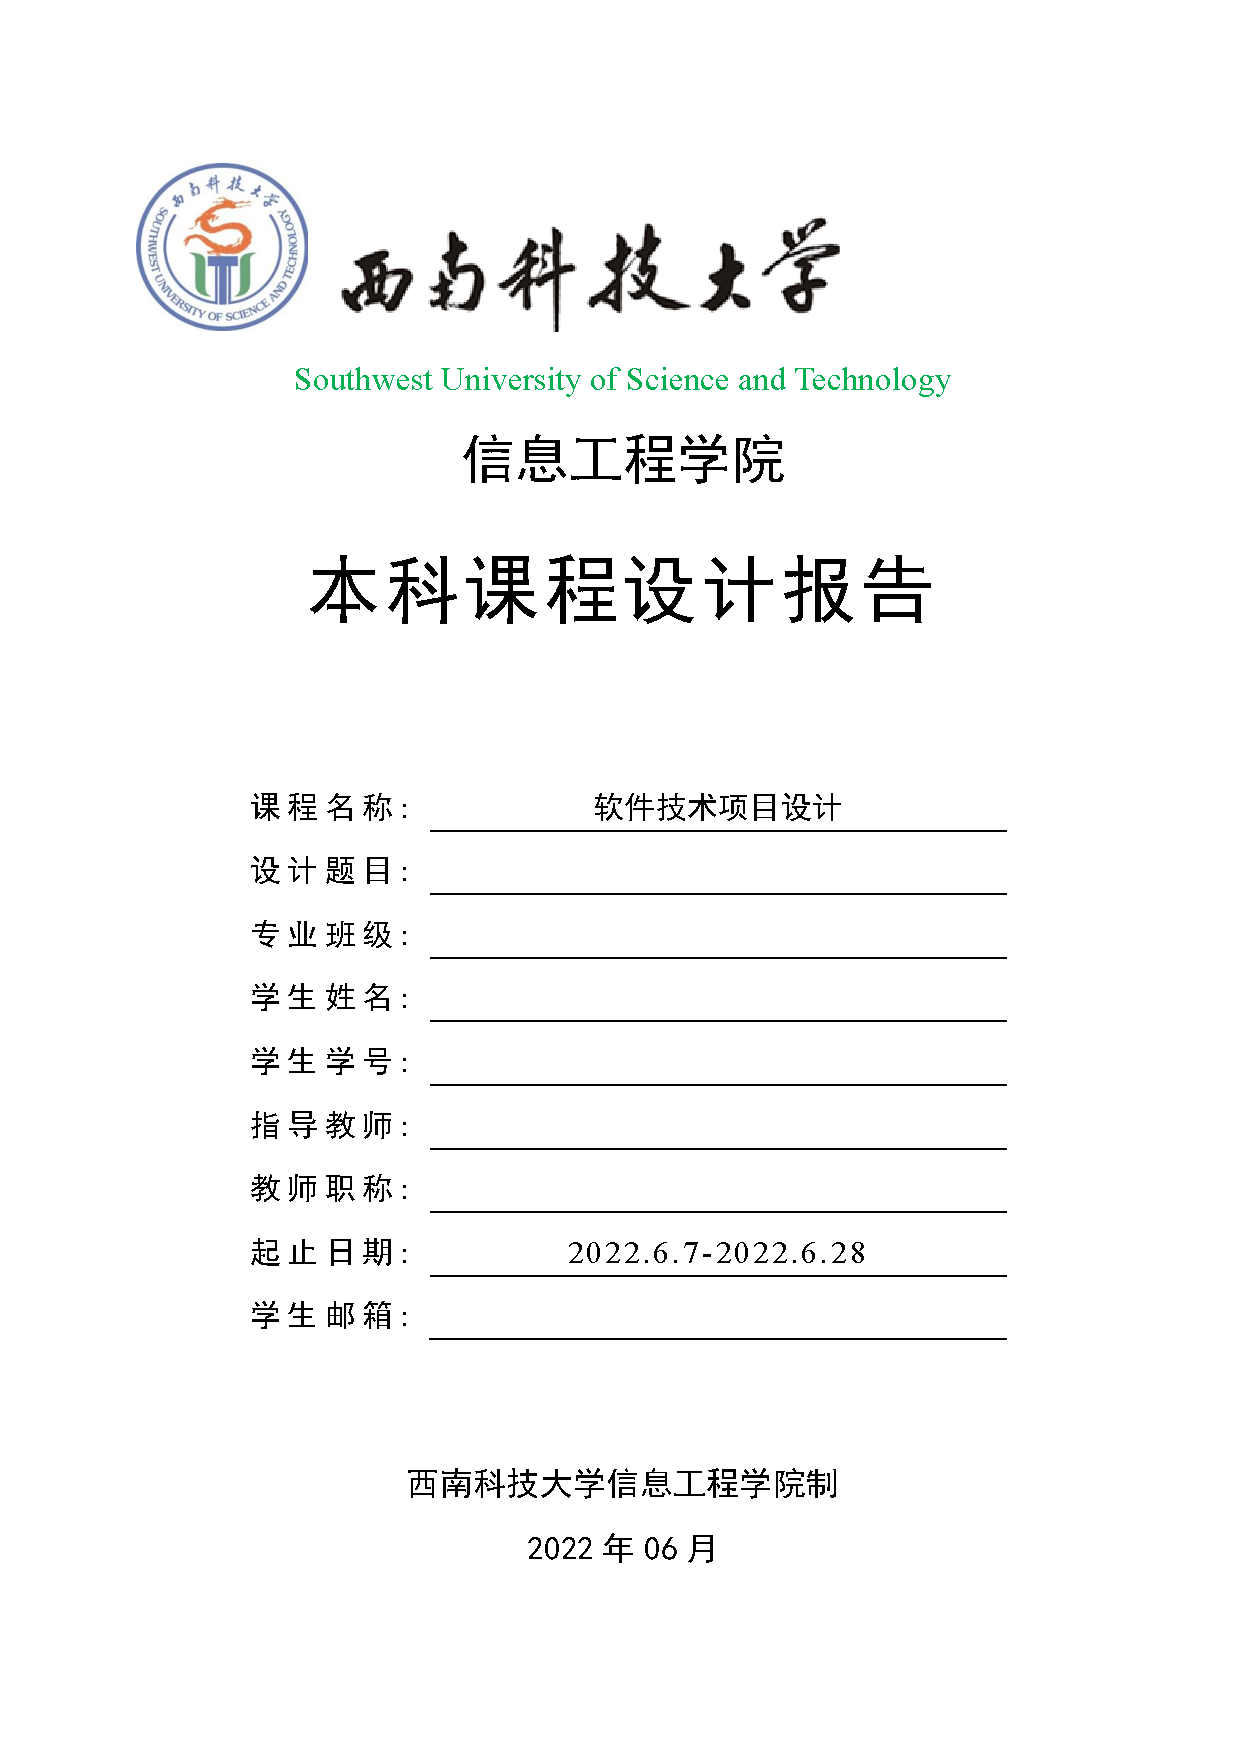
\includepdf[pages={1-4}]{MB202206.pdf}

% 生成题目
\begin{center}
\huge{\textbf{一个设计题目}}
\end{center}

\thispagestyle{empty}
\begin{abstract}
参考ccf小论文和985硕博论文。
\end{abstract}

\noindent\textbf{关键词:} 计算机视觉 \quad 卷积神经网络 \quad 目标检测 \quad \LaTeX
\newpage  % 摘要

\thispagestyle{empty}
\tableofcontents % 目录
\newpage
%% 正文开始----------------------------------------------------
\pagestyle{plain}
\setcounter{page}{1}
% ----------------------------------------------------
\section{课题重述与背景}
\subsection{文献}
baidu很多信息有缺失,建议用中文万方或cnki,英文dblp或其他出版社官网。

机器学习~\cite{qiu2020nndl}

深度学习~\cite{LeCun2015deep}

HOG~\cite{dalal2005hog}



\subsection{图}
一个简单的图实例如下图\ref{1-1}所示。
\begin{figure}[H]
\centering

\includegraphics[scale=0.2]{logo-1.png}
\caption{图标题}
\label{1-1}
\end{figure}

\subsection{公式}

质能方程:$E=mc^2$,牛顿第二定律:$a=\dfrac {d^2x}{dt^2}$和积分:
$\int^a_bx^2dx$,这几个不懂就是幼儿园民科。

公式一般都使用自动编号实例:
\begin{equation}
f(x) = a - b 
\end{equation}



\begin{equation}
  \begin{aligned}
    \sum_{k=1}^{4}x_p^k=1,\forall p\in P,
  \end{aligned}
\end{equation}

\subsection{表}


中文中的常见三线表如下表~\ref{tab:1-1}所示:

\begin{table}[!htbp]
\centering
\caption{这是一张三线表}\label{tab:1-1}%添加标题 设置标签
\begin{tabular}{ccc}
\toprule
姓名            & 学号  & 性别\\
\midrule
Steve Jobs      & 001   & Male\\
Bill Gates      & 002   & Female\\
\bottomrule
\end{tabular}
\end{table}






\clearpage


\section{课题结果}
\setcounter{figure}{0}  % 每章将图序号清零
\setcounter{table}{0}

\begin{figure}[H]
\centering

\includegraphics[scale=0.2]{logo-1.png}
\caption{图标题}
\label{2-1}
\end{figure}
一个简单的图实例如下图\ref{2-1}所示。



\clearpage 


% -------------------------------------------------------------
%\section*{参考文献}
\addcontentsline{toc}{section}{参考文献} % xelatex 编译两次
\begin{spacing}{1.0} % 行距
	\zihao{5} \songti
	\bibliography{ref}
	\vspace{11bp}
\end{spacing}

\clearpage
% ---------------------------------------------------------------------------------------
\appendix

\newpage
\section{附录一:matlab代码}

\begin{lstlisting}[language=matlab]
[X, Y] = meshgrid(0.01:0.01:1, 0.01:0.01:1);
Zfun =@(x,y)12.5*x.*log10(x).*y.*(y-1)+exp(-((25 ...
*x - 25/exp(1)).^2+(25*y-25/2).^2).^3)./25;
Z = Zfun(X,Y);
figure;
surf(Y,Z,X,'FaceColor',[1 0.75 0.65],'linestyle','none');
hold on
surf(Y+0.98,Z,X,'FaceColor',[1 0.75 0.65],'linestyle','none');
axis equal;
view([116 30]);
camlight;
lighting phong; % 设置光照和光照模式
\end{lstlisting}

\section{附录二:python代码}

\begin{lstlisting}[language=python]
def run():
from sko.GA import GA_TSP
import numpy as np
from scipy import spatial
from numpy.linalg import norm
import cvxpy as cp
import pandas as pd
#python原始代码
data=pd.read_excel("3.xlsx")
\end{lstlisting}


\end{document}
